\documentclass[letterpaper,11pt]{article}
\usepackage[spanish]{babel}
\usepackage[utf8]{inputenc}
\usepackage{graphicx}
\usepackage{amsfonts,amsmath,amssymb,float, amsthm,mathrsfs}  
\usepackage[right=4.5cm,left=2cm,top=3cm,bottom=3cm,headsep= 0.7cm,footskip=0.5cm]{geometry}
\usepackage{enumerate}
\usepackage{wrapfig} 
\usepackage[rflt]{floatflt} 
\usepackage{framed}
%\usepackage[most]{tcolorbox}
\usepackage[dvipsnames]{xcolor}
\colorlet{shadecolor}{green!20}
\setlength\FrameSep{0.5ex}
\usepackage{thmtools}
\usepackage{esint}
\usepackage{cancel}
\usepackage{listings} 
\usepackage{pstricks, caption}
\usepackage[colorlinks]{hyperref}
\usepackage{csquotes}
\usepackage{fullpage}
\usepackage{enumitem}
\usepackage{etoolbox}
\usepackage{tikz}
\usepackage{tikz-3dplot}
\tdplotsetmaincoords{80}{70}
\usetikzlibrary{decorations.markings}
\usetikzlibrary{arrows,babel}
\usepackage[font=small]{caption}
\usepackage{scalerel} %\scaleto{text}{size}
\usepackage{subcaption}
\usepackage{fancyhdr}
\usepackage{comment}
\usepackage{marginnote}
\usepackage{tensor}
\usepackage{cleveref}
\newcommand{\dbar}{\mathchar'26\mkern-12mu d}
\renewcommand*{\marginnotevadjust}{-0.1cm}
\renewcommand*{\marginfont}{\footnotesize}
\setlength{\headheight}{15pt}
\addtolength{\topmargin}{-14.49998pt}
\setlength{\headsep}{15pt}
\setlength{\footskip}{14.49998pt}
\decimalpoint
\newcommand{\grad}{^\circ}
\newlength{\drop}
\DeclareMathOperator{\sign}{sgn}
\DeclareMathOperator{\Log}{Log}
\providecommand{\norm}[1]{\lVert#1\rVert}

\let\cancelorigcolor\CancelColor% Just for conveniency...

\newcommand{\CancelTo}[3][]{%
  \ifblank{#1}{}{%
    \renewcommand{\CancelColor}{#1}%
  }
  \cancelto{#2}{#3}% 
}


\begin{document}

\pagestyle{plain}

\begin{flushleft}\vspace{-2cm}
Departamento de Física \\
Facultad de Cs. Físicas y Matemáticas\\
Universidad de Concepción
\end{flushleft}

\begin{flushright}\vspace{-1.5cm}
\textbf{Tópicos en Relatividad General} 
\end{flushright}



\rule{\linewidth}{0.1mm}

\begin{center}
\textbf{\LARGE Semana 6}
\end{center}

\begin{flushleft}
\textbf{Nombre:} Alejandro Saavedra San Martín. \\
\textbf{Profesor:} Guillermo Rubilar Alegría.
\end{flushleft}

\section*{Redshift Gravitacional}

Consideremos dos observadores en ``reposo" \ en el espaciotiempo de Schwarzschild. Desde un emisor ``escapan" \ fotones del centro de fuerzas de manera radial, ver figura \ref{fig:redshift-1}. En este caso, debido a la simetría esférica, podemos considerar que los fotones se mueven en trayectorias con $\theta = \pi/2$ y $\varphi = 0$. 

Usando la condición para curvas nulas del fotón: $g_{\mu\nu} dx^{\mu}dx^{\nu} = 0$, obtenemos que
\begin{equation}
\left(1 - \frac{2m}{r}\right) c^2dt^2 - \frac{dr^2}{\left(1 - \frac{2m}{r}\right)} = 0.
\end{equation}  

Por lo tanto, despejando $c^2dt^2$ y sacando raíz cuadrada,
\begin{equation}
c \,dt = \pm \frac{dr}{\left(1 - \frac{2m}{r} \right)}.
\end{equation} 

Los signos positivo y negativo corresponden a fotones ``escapando desde" \ y ``cayendo hacia" \ el centro de fuerzas, respectivamente. Para el primero caso, tenemos que 
\begin{equation}
c(t-t_0) = \int_{r_0}^r \frac{dr'}{\left(1 - \frac{2m}{r'}\right)} = \int_{r_0}^r \frac{r'}{r'-2m} \,dr',
\end{equation}
donde $x_{\text{i}}^{\mu} = (ct_0,r_0,\pi/2,0)$ son las coordenadas iniciales del fotón y $x_{\text{f}}^{\mu} =(ct,r,\pi/2,0)$ las finales. 

Si hacemos el cambio de variable $u = r'-2m$ tal que $du = dr'$, entonces 
\begin{align}
c(t-t_0) &= \int_{r_0 - 2m}^{r - 2m} \frac{u + 2m}{u} du \nonumber \\
&= \int_{r_0 - 2m}^{r - 2m} 1 + \frac{2m}{u} \, du\nonumber \\
&= (u + 2m\ln|u|)|_{r_0-2m}^{r - 2m}\nonumber \\
&= r - r_0 + 2m\ln\left| \frac{r-2m}{r_0-2m} \right| \nonumber\\
&= r - r_0 + 2m\ln \left(\frac{r-2m}{r_0-2m}\right),
\end{align} 
el valor absoluto se retiró, pues $r,r_0 > 2m$. Por lo tanto,
\colorlet{shadecolor}{green!20}
\begin{shaded}
\begin{equation}
ct = ct_0 +  r - r_0 + 2m \ln \left(\frac{r-2m}{r_0-2m}\right). \label{eq:trayectory-light-1}
\end{equation}
\end{shaded}

Esta relación define en forma explícita la ecuación de la trayectoria, exacta en el espaciotiempo de Schwarzschild, $r = r(t)$, del fotón escapando radialmente. 

Un dibujo esquemático de la situación física está ilustrado en la figura \ref{fig:redshift-1} y el diagrama del espacio-tiempo en la figura \ref{fig:redshift-2}. Si el emisor ubicado en $r = r_{\text{E}}$ emite un fotón en la coordenada temporal $t_{\text{E}_1}$, la ecuación de la trayectoria que sigue el fotón (en el diagrama del espaciotiempo) se obtiene al reemplazar $r_0 = r_{\text{E}}$ y $t_0 = t_{\text{E}_1}$ en \eqref{eq:trayectory-light-1}:
\begin{equation}
ct = ct_{\text{E}_1} + r - r_{\text{E}} + 2m \ln\left( \frac{r-2m}{r_{\text{E}} - 2m}\right). \label{eq:trayectory-light-2}
\end{equation}

\begin{figure}
    \centering
    \begin{subfigure}[t]{0.48\textwidth}
        \centering
        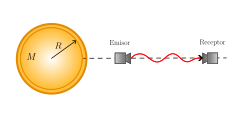
\includegraphics[width=\linewidth]{Fig-Redshift_gravitacional_1}
        \caption{Esquema de la situación física.}
        \label{fig:redshift-1}
    \end{subfigure}\hskip 1em%
    \begin{subfigure}[t]{0.48\textwidth}
        \centering
        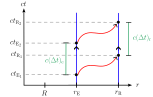
\includegraphics[width=\linewidth]{Fig-Redshift_gravitacional_2}
        \caption{Diagrama del espaciotiempo.}
        \label{fig:redshift-2}
    \end{subfigure}
\end{figure}

Si se emite otro fotón en la coordenada temporal $t_{\text{E}_2}$, la ecuación de la trayectoria es
\begin{equation}
ct = ct_{\text{E}_2} + r - r_{\text{E}} + 2m \ln\left( \frac{r-2m}{r_{\text{E}} - 2m}\right). \label{eq:trayectory-light-3}
\end{equation}

Si $c(\Delta t)_{\text{e}} = ct_{\text{E}_2} - ct_{\text{E}_1}$, entonces \eqref{eq:trayectory-light-3} nos queda
\begin{equation}
ct = ct_{\text{E}_1} + c(\Delta t)_{\text{e}} + r - r_{\text{E}} + 2m \ln\left( \frac{r-2m}{r_{\text{E}} - 2m}\right). \label{eq:trayectory-light-4}
\end{equation}

El primer fotón llega al receptor ($r = r_{\text{R}}$) en la coordenada temporal $t_{\text{R}_1}$  y el segundo fotón en la coordenada temporal $t_{\text{R}_2}$. Reemplazando estos datos en \eqref{eq:trayectory-light-2} y \eqref{eq:trayectory-light-4}, respectivamente,
\begin{align}
ct_{\text{R}_1} &=  ct_{\text{E}_1} + r_{\text{R}} - r_{\text{E}} + 2m \ln\left( \frac{r_{\text{R}}-2m}{r_{\text{E}} - 2m}\right), \label{eq:trayectory-light-5} \\
ct_{\text{R}_2} &=  ct_{\text{E}_1} + c(\Delta t)_{\text{e}} + r_{\text{R}} - r_{\text{E}} + 2m \ln\left( \frac{r_{\text{R}}-2m}{r_{\text{E}} - 2m}\right). \label{eq:trayectory-light-6}
\end{align}

Si $c(\Delta t)_{\text{r}} = ct_{\text{R}_2} - ct_{\text{R}_1}$, entonces
\begin{equation}
(\Delta t)_{\text{r}} = (\Delta t)_{\text{e}}.
\end{equation}

Este es un resultado general, válido para todo espaciotiempo estacionario. Por ejemplo, si consideramos el elemento de línea
\begin{equation}
ds^2 = A(r) c^2 dt^2 - B(r) dr^2 - r^2 [d\theta^2 + \sin^2\theta d\varphi^2],
\end{equation}
donde $A(r)$ y $B(r)$ son funciones de la coordenada radial $r$.

Usando la condición $g_{\mu\nu} dx^{\mu}dx^{\nu} = 0$ y fijando $\theta = \pi/2$ y $\varphi = 0$, obtenemos que
\begin{equation}
A(r) c^2dt^2 - B(r) dr^2 = 0.
\end{equation} 

Luego,
\begin{equation}
c\,dt = \pm \sqrt{\frac{B(r)}{A(r)}} dr,
\end{equation}
siempre que $B/A > 0$. Si consideramos el caso con $+$ y que las coordenadas iniciales del fotón son $x_{\text{i}}^{\mu} = (ct_0,r_0,\pi/2,0)$ y finales $x_{\text{f}}^{\mu} = (ct,r,\pi/2,0)$, la ecuación de la trayectoria nos queda
\begin{equation}
ct = ct_0 + \int_{r_0}^{r} \sqrt{\frac{B(r')}{A(r')}} dr'.
\end{equation}

Bajo la misma situación física de dos fotones emitidos en $r = r_{\text{E}}$ a diferentes coordenadas temporales, $t_{\text{E}_1}$ y $t_{\text{E}_2}$, y recibidos en $r = r_{\text{R}}$ en coordenadas temporales $t_{\text{R}_1}$ y $t_{\text{R}_2}$, respectivamente, obtenemos que
\begin{align}
ct_{\text{R}_1} &=  ct_{\text{E}_1} + \int_{r_{\text{E}}}^{r_{\text{R}}} \sqrt{\frac{B(r')}{A(r')}} dr', \label{eq:trayectory-light-7} \\
ct_{\text{R}_2} &=  ct_{\text{E}_1} + c(\Delta t)_{\text{e}} +\int_{r_{\text{E}}}^{r_{\text{R}}} \sqrt{\frac{B(r')}{A(r')}} dr'. \label{eq:trayectory-light-8}
\end{align}

Por lo tanto,
\begin{equation}
c(\Delta t)_{\text{r}} = ct_{\text{R}_2} - ct_{\text{R}_1} = c(\Delta t)_{\text{e}}. 
\end{equation}

Es importante recordar que lo único medible es el tiempo propio, entonces el resultado $c(\Delta t)_{\text{r}}  = c(\Delta t)_{\text{e}}$ no significa que los fotones son recibidos en el mismo intervalo que se emitieron. Recordemos que 
\begin{equation}
c\,d\tau = \sqrt{g_{\mu\nu} dx^{\mu}dx^{\nu}}.
\end{equation}

Así, los tiempos propios asociados a observadores ``en reposo"\ en el punto de emisión y recepción, es decir, cuyas líneas de mundo tienen coordenada radial constante $r_{\text{E}}$ y $r_{\text{R}}$, respecitvamente, quedan determinados por 
\begin{equation}
c\, d\tau = \sqrt{1 - \frac{2m}{r}} c\,dt,
\end{equation}
de modo que
\begin{equation}
\Delta \tau_{\text{e}} = \sqrt{1 - \frac{2m}{r_{\text{E}}}} (\Delta t)_{\text{e}}, \quad \Delta \tau_{\text{r}} = \sqrt{1 - \frac{2m}{r_{\text{R}}}} (\Delta t)_{\text{r}}.
\end{equation}

Con estos ingredientes, obtenemos
\begin{shaded}
\begin{equation}
\frac{\Delta \tau_\text{r}}{\Delta \tau_{\text{e}}} = \sqrt{\frac{1 - \frac{2m}{r_{\text{R}}}}{1 - \frac{2m}{r_{\text{E}}}}}. \label{eq:redshift-grav}
\end{equation}
\end{shaded}

En el límite de campo débil: $r_{\text{E}}, r_{\text{R}} \gg 2m$, se tiene que
\begin{equation}
\frac{1}{1 - \frac{2m}{r_{\text{E}}}} = 1 + \frac{2m}{r_{\text{E}}} + \mathcal{O}\left(\frac{4m^2}{r_{\text{E}}^2} \right).
\end{equation}

Luego, a primer orden en $2m/r_{\text{E}}$ y $2m/r_{\text{R}}$,
\begin{align}
\frac{1 - \frac{2m}{r_{\text{R}}}}{1 - \frac{2m}{r_{\text{E}}}} &= \left( 1 - \frac{2m}{r_{\text{R}}} \right) \left( 1 + \frac{2m}{r_{\text{E}}} + \mathcal{O}\left(\frac{4m^2}{r_{\text{E}}^2} \right) \right)  \nonumber\\
&\approx 1 + \frac{2m}{r_{\text{E}}} - \frac{2m}{r_{\text{R}}}.
\end{align}

Reemplazando en \eqref{eq:redshift-grav} y expandiendo en serie de Taylor:
\begin{equation}
\frac{\Delta \tau_\text{r}}{\Delta \tau_{\text{e}}} \approx \sqrt{1 + \frac{2m}{r_{\text{E}}} - \frac{2m}{r_{\text{R}}}} \approx 1 + \frac{m}{r_{\text{E}}} - \frac{m}{r_{\text{R}}}.
\end{equation}

Si $\Delta \tau_{\text{e}}$ corresponde al periodo de emisión $P_{\text{e}}$ de una onda y $\Delta \tau_{\text{r}}$ corresponde al periodo de recepción $P_{\text{r}}$, tenemos que
\begin{equation}
\frac{\Delta \tau_\text{r}}{\Delta \tau_{\text{e}}} = \frac{P_{\text{e}}}{P_{\text{r}}} = \frac{\nu_{\text{r}}}{\nu_{\text{e}}} = \frac{\lambda_{\text{r}}}{\lambda_{\text{e}}}. 
\end{equation}

Como el redshift está dado por
\begin{equation}
z = \frac{\lambda_{\text{r}} - \lambda_{\text{e}}}{\lambda_{\text{e}}} = \frac{\lambda_{\text{r}}}{\lambda_{\text{e}}} - 1,
\end{equation}
encontramos, en Relatividad General, que
\begin{equation}
z = \sqrt{\frac{1 - \frac{2m}{r_{\text{R}}}}{1 - \frac{2m}{r_{\text{E}}}}} - 1
\end{equation}
y en el límite de campo débil,
\begin{equation}
z \approx \frac{m}{r_{\text{E}}} - \frac{m}{r_{\text{R}}} = \frac{GM}{c^2 r_{\text{E}}} - \frac{GM}{c^2 r_{\text{R}}} = \frac{\Delta \phi}{c^2},
\end{equation}
donde $\phi(r) = - GM/r$. Resultado que coincide con lo visto para el redshift gravitacional no relativista (Newton + principio de equivalencia fuerte).
\end{document}
